\section{Постановка задачи детектирования фазоманипулированного сигнала с расширенным спектром}
Широкополосными сигналами (ШПС) - сигналы, ширина полосы, используемой для передачи сигнала, которых
намного шире минимальной, необходимой для передачи данных \cite{sklyar}. Система связи считается системой с расширенным
спектром в следующих случаях \cite{sklyar}:

\begin{enumerate}
	\item Используемая полоса значительно шире минимальной, необходимой для передачи данных.
	\item Расширение спектра производится с помощью так называемого расширяющего (кодового) сигнала,
		который не зависит от передаваемой информации.
	\item Восстановление исходных данных ("сужение спектра") осуществляется путем сопостовления полученного
		сигнала и синхронизированной копии расширяющего сигнала
\end{enumerate}
Так же подобные сигналы называют:
\textquotedblleftсложными\textquotedblright,
\textquotedblleftшумоподобными\textquotedblright,
\textquotedblleftпсевдослучайными\textquotedblright,
\textquotedblleftсложными-дискретными\textquotedblright,
\textquotedblleftдискретно-кодированными\textquotedblright,
\textquotedblleftортогональными (квазиортогональными)\textquotedblright,
\textquotedblleftоптимальными дискретными\textquotedblright
\cite{gantmaher-book}.
Каждое название ставит акцент на определенной характеристике сигнала. В данной работе я буду оперировать термином
широкополосный сигнал - ШПС. ШПС можно определить как \cite{gantmaher-book, varakin-book}:

\begin{center}
\begin{equation}
	\label{eq:ss_signal}
	1 << FT = B,
\end{equation}
\end{center}
где: ${B}$ - база сигнала, ${F}$ - эффективная ширина спектра, а ${T}$ - длительность.
Неточность этого определеная рассмотрена в \cite{gantmaher-book}, так же там даны ссылки на другие источники
разделяющие критику данного определения. Для данной работы данная критика принципального значения не имеет.

В данной работе используется сигнал с расширенным спектром методом "прямой последовательности". Данный метод
заключается в том, что несущая сигнала модулируется высокоскоростным (широкополосным) расширяющим сигналом \cite{sklyar}.
Методы генерации таких последовательностей рассмотрены, например, в \cite{gantmaher-book}. Это отдельная большая
тема для исследований. В данной работе используется ПСП - код Гоулда. Свойства данной ПСП подробно рассмотрены в
\cite{gold-ieee}, а так же краткое описание свойств без доказательства приведены в \cite{tsui, akos-book}.

Метод генерирования ПСП подробно рассмотрен во многих источниках \cite{tsui, akos-book, kaplan}
и в данной работе рассматриваться не будет. Определим входной сигнал как \cite{akos-book}:

\begin{center}
\begin{equation}
	\label{eq:gps_signal}
	s_k(t) = \sqrt{2A}(C_k(t) * D_k(t)) + \cos(2\pi{f})
\end{equation}
\end{center}
где: ${A}$ - мощность сигнала, ${C_k}$ - ПСП для ${k}$ - сигнала, ${D}$ - данные, а ${f}$ - частота несущей сигнала.

\begin{figure}[H]
\center\scalebox{0.5}{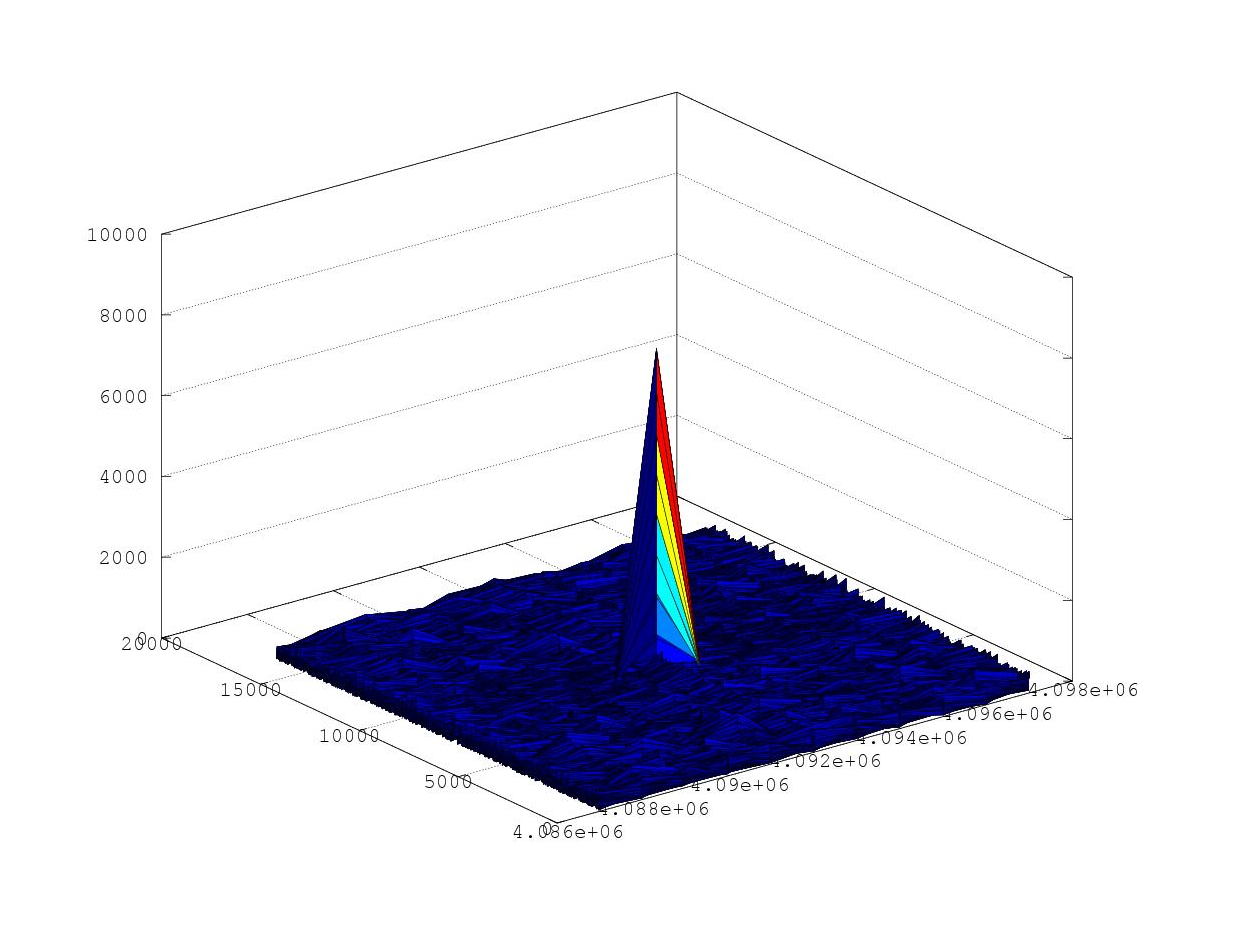
\includegraphics[width=1\linewidth]{corr_peak.eps}}
\caption{График ФН}
\label{pic:corr_peak}
\end{figure}

Задача поиска сигнала сводится к устранению неопределенности по двум параметрам: центральной частоте его спектра
и фазе ПСП. На рисунке \ref{pic:ambiguity_region} представлена область неопределенности. Можно заметить, что сечение
области неопределенности плоскостью ${f}$ представляет собой КФ сигнала. Поиск сигнала соответствует поиску и
оценке основного пика КФ.

\begin{figure}[H]
\center\scalebox{0.5}{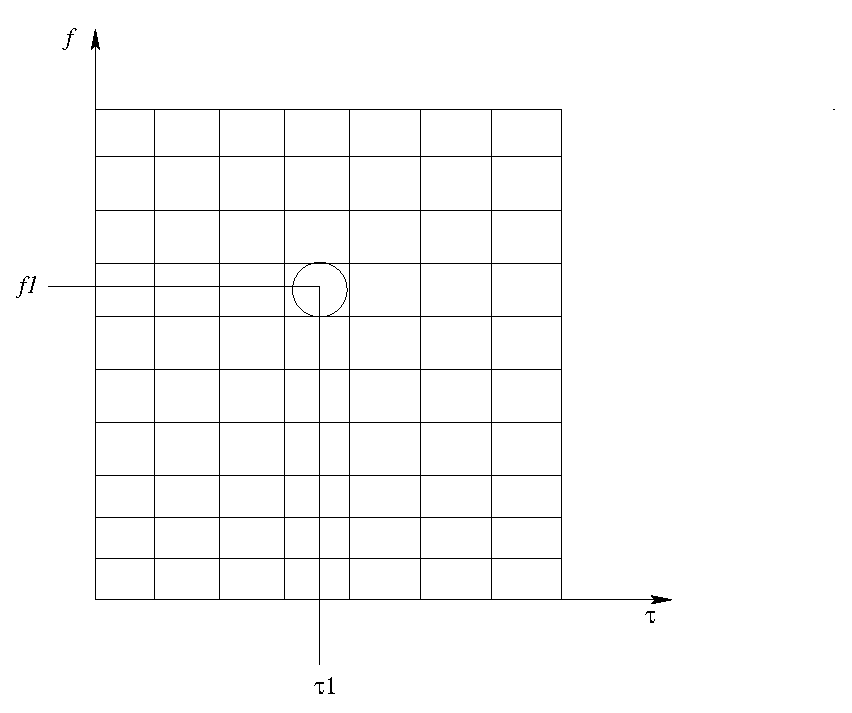
\includegraphics[width=1\linewidth]{ambiguity_region.eps}}
\caption{Область неопределенности}
\label{pic:ambiguity_region}
\end{figure}

\newpage
